\documentclass[10pts]{article}

%% Language and font encodings
\usepackage[english]{babel}
\usepackage[utf8x]{inputenc}
\usepackage[T1]{fontenc}
\usepackage{float}
\usepackage{listings}
\usepackage{nicefrac}
%% Sets page size and margins
\usepackage[letterpaper,top=3cm,bottom=2cm,left=3cm,right=3cm,marginparwidth=1.75cm]{geometry}

%% Useful packages
\usepackage{amsmath}
\usepackage{amsthm}
\usepackage{graphicx}
\usepackage{subcaption}
\usepackage{color}
\usepackage{xcolor}
\usepackage[colorlinks,allcolors=blue]{hyperref}
\usepackage{cleveref}
\usepackage{booktabs}
\usepackage{multirow}
\usepackage{paralist}
\usepackage{cite}
%\definecolor{codegreen}{rgb}{0,0.6,0}
%\definecolor{codegray}{rgb}{0.5,0.5,0.5}
%\definecolor{codepurple}{rgb}{0.58,0,0.82}
%\definecolor{backcolour}{rgb}{0.95,0.95,0.92}

\newif\ifdraft
\drafttrue
\ifdraft
\definecolor{ocolor}{rgb}{1,0,0.4}
\newcommand{\jwave}[1]{ {\reduwave{#1}}}
\newcommand{\jhanote}[1]{ {\textcolor{red} { ***shantenu: #1 }}}
\newcommand{\mtnote}[1]{ {\textcolor{cyan} { ***matteo: #1 }}}
\definecolor{orange}{rgb}{1,.5,0}
\definecolor{dandelion}{cmyk}{0,0.29,0.84,0}
\newcommand{\gpnote}[1]{{\textcolor{green} {***giannis: #1}}}
\newcommand{\note}[1]{ {\textcolor{magenta} { ***Note: #1 }}}
\else
\newcommand{\jwave}[1]{}
\newcommand{\jhanote}[1]{}
\newcommand{\mtnote}[1]{}
\newcommand{\gpnote}[1]{}
\newcommand{\note}[1]{}
\fi

\theoremstyle{definition}
\newtheorem{defn}{Definition}[section]

\lstdefinestyle{mystyle}{
    backgroundcolor=\color{backcolour},   
    commentstyle=\color{codegreen},
    keywordstyle=\color{magenta},
    numberstyle=\tiny\color{codegray},
    stringstyle=\color{codepurple},
    basicstyle=\footnotesize,
    breakatwhitespace=false,         
    breaklines=true,                 
    captionpos=b,                    
    keepspaces=true,                 
    numbers=left,                    
    numbersep=5pt,                  
    showspaces=false,                
    showstringspaces=false,
    showtabs=false,                  
    tabsize=2
}
 
\lstset{style=mystyle}

\title{Campaign manager for executing scientific campaigns on High Performance 
Computing resources}\author{Ioannis Paraskevakos}
\author{Ioannis Paraskevakos}
\vspace{-8ex}
\date{}

\begin{document}
\maketitle

Progress in many scientific problems requires executing an increasing number of 
computational workflows to achieve scientific insight. We are motivated by 
workflows of ensembles of up to $O(10^5)$ computational tasks from ecological 
and biomolecular domains, organized in up to $O(10^3)$ 
pipelines~\cite{rietmann2012forward, dakka2018high, paraskevakos2019workflow} 
with heterogeneous resource requirements. Based on our use cases, a set of 
workflows is required to be executed, where each workflow can process and/or 
produce 100TB of data and execute tasks running for up to 24 hours. This set 
of workflows, with or without dependencies amongst them, constitutes a 
computational campaign. Effective and efficient execution of computational 
campaigns requires resource management and coordination at runtime.

A computational campaign is a set of heterogeneous workflows, with or without 
dependencies amongst them, that need to be executed. Workflows are heterogeneous 
when they have to either perform different types of work and/or have different 
resource requirements. We identify three types of dependencies between workflows 
in a campaign:
\begin{inparaenum}[1)]
\item data dependencies, 
\item temporal dependencies, and 
\item resource sharing dependencies
\end{inparaenum}. 
Temporal dependencies refer either to a temporal order between workflows or to 
a moment in time where the workflow can be executed. Resource sharing 
dependencies between workflows refer to workflows executing in the same resource 
concurrently given sufficient capacity or interchangeably. For a set of 
workflows to be categorized as a campaign it should have at least ten workflows.

Workflows are mainly executed by utilizing dedicated workflow management 
frameworks~\cite{balasubramanian2018harnessing,deelman2015pegasus,ludascher2006scientific,rocklin2015dask,airflow}. 
Currently, workflow management frameworks offer a vast array of capabilities 
but, tend to lack campaign planning and execution capabilities. Campaign planning 
and execution requires scheduling workflows to resources, resolving dependencies 
between workflows, as well as managing the execution of the campaign. As a result, 
when executing a computational campaign, users have to derive, execute and often 
adapt campaign execution plans, manually solving scheduling problems, satisfying 
dependencies, and managing workflow executions. Thus, a campaign manager to 
automatically derive, execute and adapt an execution plan is desirable.

Resources, workflows and campaigns can either be static or dynamic. A resource 
is considered static when its performance is constant over time, or dynamic when 
it changes. A workflow can be known \textit{a-priori}, i.e. all tasks and 
dependencies described, and thus static~\cite{paraskevakos2019workflow}, or 
change during runtime by adding tasks and dependencies, thus dynamic~\cite{dakka2018high}. 
Accordingly, when the set of workflows, and their dependencies, that comprise 
the campaign is known \textit{a-priori}, the campaign is considered static, and 
when the set of workflows change, by adding workflows, it is considered dynamic.

Computational campaigns enact an execution plan to allow users to achieve an 
objective under given requirements and constraints. A computational objective is 
a set of values selected by the user for a set of metrics, such as time to 
completion and throughput. This objective can then be represented as an objective 
function. Requirements describe the minimum amount and type of resources needed 
to execute each workflow of the campaign, while constraints are the conditions 
that bound the execution of the campaign, including but not limited to, resource 
availability, capacity, and costs. A plan describes a sequence of actions such 
as selecting, acquiring and configuring resources, that solve the objective 
function, as well as dependency resolution.

Planning the execution and executing a computational campaign poses three main 
challenges: 
\begin{inparaenum}[(i)]
\item evaluate the time needed to execute all the workflows, i.e. makespan, of 
a campaign on heterogeneous and dynamic resources,
\item determining a campaign execution plan (workflows’ execution order, 
workflows’ resource mapping) on available resources that satisfies the objective 
function while being subject to the requirements and constraints of a campaign, 
and
\item adapting the plan in case of deviating from the objective achievement.
\end{inparaenum}

In accordance with those challenges and within the requirements of our target 
use cases, this work will offer three main contributions: 
\begin{inparaenum}[(1)]
\item an algorithm to calculate the makespan of a campaign on heterogeneous 
resources;
\item a software system that implements the makespan algorithm, and executes a 
campaign on resources; and 
\item a method to evaluate the performance of our approach compared to a random 
plan. 
\end{inparaenum}
Compared to existing solutions, our research will allow users to execute 
campaigns that contain $O(10)$ workflows with $O(1000)$ tasks. We will implement 
these contributions into a software prototype designed to execute ecological 
and biomolecular use cases on high performance computing (HPC) resources, using 
an existing workflow execution framework as implemented by RADICAL-EnsembleToolkit 
(EnTK)~\cite{balasubramanian2018harnessing}.

The makespan of a campaign is the time needed to execute all the workflows of 
the campaign, or alternatively, the maximum execution time among all paths 
throughout the campaign~\cite{chirkin2017execution}. Several methods have been 
proposed~\cite{lu2019review} to calculate the makespan of a workflow, including 
queuing network~\cite{yao2019throughput,bao2019performance}, and domain specific 
languages~\cite{carothers2017durango,maheshwari2016workflow}. We propose to 
extend the Heterogeneous Earliest Finish Time (HEFT)~\cite{topcuoglu2002performance} 
algorithm to calculate the makespan and schedule of a computational campaign. 
Among the alternatives to HETF, queuing networks is likely to be of limited use 
because they require the user to provide an equivalent queuing network of the 
workflow; domain specific languages approaches would require too much engineering 
effort to convert a workflow representation based on domain specific assumptions, 
e.g. MPI style workflow, or specific languages representation, e.g Swift.

HEFT~\cite{topcuoglu2002performance} is an offline scheduling algorithm which 
calculates the makespan of a workflow on heterogeneous resources. HEFT uses a 
matrix to represent execution time of tasks on resources. HEFT assigns tasks to 
the resource that minimizes the finish time of the task. HEFT has complexity 
proportional to the number of dependencies between tasks and the number of 
resources offered. Furthermore, there has been some initial research to extend 
HEFT to resources that provide CPU and GPUs~\cite{shetti2013optimization}. 

Calculating the makespan of a computational campaign depends on workflow 
characteristics, workflow dependencies, campaign dynamicity, and resource 
availability and dynamicity. Task execution time depends on parallelism, 
coordination between tasks, task characteristics~\cite{khoshlessan2017parallel}, 
the framework used to support task execution~\cite{paraskevakos2018task}, and 
resource dynamicity~\cite{paraskevakos2019workflow}. We propose to utilize 
approximations of workflow execution time that we will experimentally derive.

Based on workflow tasks’ characteristics, resources may need to be configured 
with different execution engines. Compute intensive tasks on HPC resources are 
mainly executed via OpenMP/MPI benefitting from parallelism at scale, while data 
intensive tasks via data parallel frameworks such as Hadoop, Spark~\cite{zaharia2010spark}, 
or Dask~\cite{rocklin2015dask}. Traditionally, HPC resources are designed to 
optimize the execution of MPI tasks, leaving data-parallel frameworks largely 
unsupported. In Ref.~\cite{luckow2016hadoop}, we show how a pilot-based 
middleware~\cite{merzky2019using} can support the efficient and scalable execution 
of data-parallel applications on HPC resources. Such capabilities are necessary 
to support and plan the execution of a data-intensive campaign.

\begin{figure}[t]
	\centering
	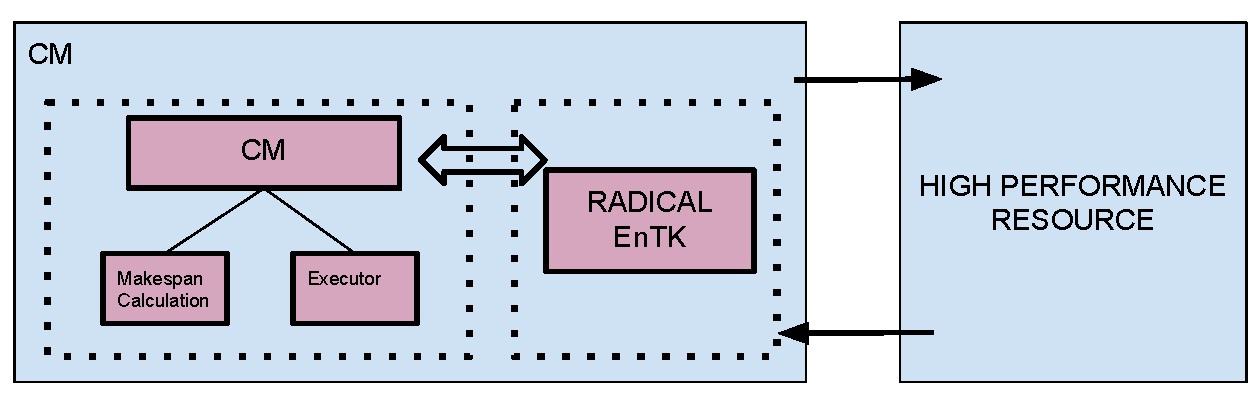
\includegraphics[width=.85\textwidth]{CEM_RefArch.pdf}
    \caption{Reference Architecture of a Campaign Execution Manager. Basic 
    components of Campaign Execution Framework (CEF): 1) Campaign Execution 
    Manager, subcomponents: i) Makespan Calculation, and Campaign, 2) Executor. 
    CEM communicates decisions to RADICAL-EnTK. CEF communicates with HPCs to 
    execute parts of the campaign.}\label{refarch}
\end{figure}

We propose to define a campaign manager (CM) which, given a campaign, an objective, 
and a set of constraints, can derive an execution plan by utilizing the proposed 
makespan methods. Figure~\ref{refarch} shows a reference architecture of the proposed 
framework.We propose to define a campaign manager (CM). CM has two sub-components: 
\begin{inparaenum}[(1)]
\item Makespan Calculation which implements the proposed makespan algorithm, and 
\item an Executor which executes the plan. Workflow execution is done through 
RADICAL-EnTK to HPC resources
\end{inparaenum}.
Based on workflows metrics, such as tasks execution time, overheads calculation 
and time to completion, provided by EnTK,  and as a consequence the respective 
workflows and campaign metrics, CEM will adapt the execution plan if necessary 
by updating the workflows to resource mapping decisions.

To understand the performance of the proposed approach, we will compare it with 
a randomly decided execution plan. We propose to model a random decision as the 
mapping of a campaign’s workflows to resources based on a uniform distribution 
between resources. The random plan provides a baseline of performance. Based on 
this comparison, we will be able to validate whether our approach offered better 
performance, i.e. smaller makespan after execution, as well as to better 
understand the problem’s requirements for further research and development.

Given the size of the problem space and that the proposed work will be performed 
in no more than one year, we propose to focus on the three main contributions 
described above. In more detail, we will focus on: 
\begin{inparaenum}[(1)]
\item evaluating and deriving the makespan for a campaign as a set of independent 
static O(10) workflows with heterogeneous resource requirements provided by 
ecological and biomolecular sciences use cases on static resources; 
\item offering execution planning capabilities to minimize the makespan of a 
campaign; and 
\item validating our planning capability by executing the workflows of our use 
cases and measuring the accuracy of the estimated campaign runtime and planned 
execution
\end{inparaenum}. In addition, we will explore the requirements to support 
execution plan adaptivity.

To this end, we propose to achieve the following objectives with an estimation 
of the time needed:
\begin{enumerate}
    \item Derive the makespan for a campaign from the ecological sciences. 
    Durations 3 months.
    \item Develop a campaign manager, which will derive and execute a plan 
    based on the results of objective 1. Duration 4 months, overlap with the 
    last month of objective 1.
    \item Integration with scientific workflows and experimentally validate the 
    plan by measuring the average deviation of the manager from the optimal 
    objective. Duration 4 months. The first two months overlap with objective 2.
\end{enumerate}
\bibliographystyle{unsrt}
\bibliography{ext}
\end{document}